\documentclass[conference]{IEEEtran}
\IEEEoverridecommandlockouts

\usepackage[utf8]{inputenc}
\usepackage[T1]{fontenc}
\usepackage{cite}
\usepackage{amsmath,amssymb,amsfonts}
\usepackage{algorithmic}
\usepackage{graphicx}
\usepackage[caption=false,font=footnotesize]{subfig} % subfiguras compatibles con IEEEtran
\usepackage[section]{placeins} % evita que los floats se vayan a secciones/subsecciones posteriores
\usepackage{textcomp}
\usepackage{xcolor}
\usepackage{url}
\usepackage{booktabs}

\def\BibTeX{{\rm B\kern-.05em{\sc i\kern-.025em b}\kern-.08em
    T\kern-.1667em\lower.7ex\hbox{E}\kern-.125emX}}

\begin{document}

\title{Predicción de Mortalidad Hospitalaria mediante Machine Learning con el Dataset SUPPORT}

\author{
\IEEEauthorblockN{1\textsuperscript{st} Joaquin Geronimo Arriaga Cosio}
\IEEEauthorblockA{
\textit{Ciencia de la Computación} \\
\textit{Universidad de Ingeniería y Tecnología (UTEC)} \\
Lima, Perú
}
\and

\IEEEauthorblockN{2\textsuperscript{nd} Marialejandra Bautista Gastelo}
\IEEEauthorblockA{
\textit{Ciencia de la Computación} \\
\textit{Universidad de Ingeniería y Tecnología (UTEC)} \\
Lima, Perú
}
\and

\IEEEauthorblockN{\makebox[\linewidth][c]{3\textsuperscript{rd} Elizabeth Huaman Santillan}}
\IEEEauthorblockA{\parbox{\linewidth}{\centering
\textit{Ciencia de la Computación} \\
\textit{Universidad de Ingeniería y Tecnología (UTEC)} \\
Lima, Perú
}}
}

\maketitle

\begin{abstract}
Se estudia la predicción de la mortalidad hospitalaria (\texttt{hospdead}) en 9105 pacientes gravemente enfermos del estudio SUPPORT a partir de variables demográficas, clínicas y fisiológicas registradas en el tercer día del estudio. Tras excluir variables con fuga de información (desenlaces, costos, puntuaciones pronósticas y órdenes de no reanimación), se compararon un baseline de clase mayoritaria, regresión logística regularizada, un árbol de decisión, Random Forest y Gradient Boosting. Los hiperparámetros se ajustaron con validación cruzada estratificada de 5 folds sobre el conjunto de entrenamiento (80\,\%), y la partición de prueba (20\,\%) se usó una sola vez. Gradient Boosting, seleccionado por ROC-AUC en validación cruzada, alcanzó en prueba un ROC-AUC de 0.834 (IC 95\,\%: 0.814--0.854) y un AP de 0.655, con buena calibración; Random Forest fue estadísticamente equivalente. Un modelo con solo variables demográficas obtuvo un ROC-AUC de 0.567, y la incorporación de las variables fisiológicas lo elevó en 0.19, lo que confirma que estas concentran la capacidad predictiva. Se analizaron además estrategias de imputación, la recalibración de los modelos con pesos de clase, umbrales de decisión con costos clínicos explícitos y por grupo diagnóstico, la importancia de variables y los errores por subgrupo. Los resultados corresponden a una clasificación retrospectiva y no constituyen una validación clínica.
\end{abstract}

\begin{IEEEkeywords}
Machine Learning, mortalidad hospitalaria, SUPPORT, variables fisiológicas, Gradient Boosting, calibración, umbral sensible al costo.
\end{IEEEkeywords}

\section{Introducción y formulación del problema}
La estimación temprana del riesgo de mortalidad en pacientes hospitalizados es un problema central en la medicina crítica, ya que orienta decisiones clínicas, la comunicación con pacientes y familiares, y la asignación de recursos hospitalarios. El estudio SUPPORT fue diseñado precisamente para mejorar la toma de decisiones en el cuidado de pacientes con enfermedades graves, mediante la construcción de modelos pronósticos objetivos basados en variables fisiológicas y clínicas \cite{knaus1995}.

En este proyecto se plantea la siguiente tarea de Machine Learning: dado un conjunto de variables demográficas, de comorbilidad y fisiológicas registradas durante los primeros días del estudio, predecir si el paciente fallecerá durante la hospitalización (variable \texttt{hospdead}). Se trata de una clasificación binaria supervisada con clase positiva $y=1$ (fallecimiento).

\textbf{Pregunta de investigación:} ?`En qué medida las variables fisiológicas registradas el día 3 del estudio permiten predecir la mortalidad hospitalaria con mayor capacidad discriminativa que las variables puramente demográficas (edad, sexo, raza, ingreso y educación)?

\textbf{Hipótesis:} se espera que los modelos que incorporan variables fisiológicas (por ejemplo, estado de conciencia, presión arterial media o función renal) superen sustancialmente a un baseline demográfico, dado que reflejan directamente la severidad clínica del paciente.

\section{Datos y Análisis Exploratorio de Datos (EDA)}

\subsection{Descripción del dataset}
Se utilizó el dataset \textit{support2}, correspondiente al estudio SUPPORT (Study to Understand Prognoses Preferences Outcomes and Risks of Treatment) \cite{supportdata}. El conjunto contiene 9105 observaciones correspondientes a pacientes hospitalizados con enfermedades graves y un total de 47 variables de naturaleza demográfica, clínica, fisiológica y pronóstica.

Cada observación representa a un paciente. Entre las variables disponibles se encuentran edad, sexo, raza, diagnóstico principal, número de comorbilidades y diferentes mediciones fisiológicas, como presión arterial media, frecuencia cardíaca, frecuencia respiratoria, temperatura, razón PaO$_2$/FiO$_2$, albúmina, bilirrubina, creatinina, sodio, glucosa, BUN y recuento de leucocitos. Según la documentación del estudio, la mayoría de las evaluaciones se realizaron en el tercer día del estudio \cite{supportdata}.

La variable objetivo seleccionada fue \texttt{hospdead}, de naturaleza binaria, donde el valor 1 representa el fallecimiento del paciente durante la hospitalización y el valor 0 indica que el paciente sobrevivió al periodo hospitalario.

\subsection{Análisis de valores faltantes}
Como parte del análisis inicial de calidad de datos, se cuantificó la cantidad y proporción de valores faltantes para cada variable. Este análisis es especialmente relevante debido a que varias variables fisiológicas y clínicas presentan observaciones incompletas.

Se calculó el porcentaje de datos faltantes respecto del total de 9105 pacientes y se ordenaron las variables de mayor a menor proporción de ausencia. Esto permite identificar aquellas características cuya utilización puede requerir estrategias específicas de imputación o, en casos de ausencia excesiva, evaluar su conveniencia dentro del conjunto de predictores.

\begin{figure}[!t]
\centering
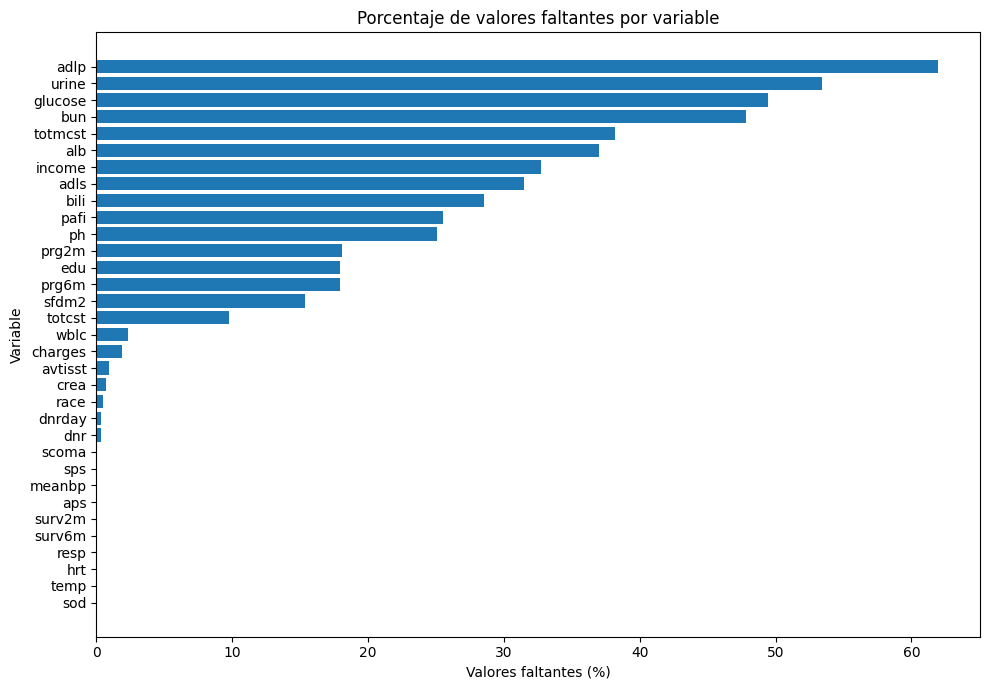
\includegraphics[width=\columnwidth]{figures/image9.png}
\caption{Proporción de valores faltantes por variable en el dataset SUPPORT.}
\label{fig:missingness}
\end{figure}
\FloatBarrier

Las variables con mayor proporción de ausencia son \texttt{adlp}, \texttt{urine}, \texttt{glucose}, \texttt{bun}, \texttt{totmcst}, \texttt{alb} e \texttt{income}. En el EDA no se imputaron datos para no alterar las distribuciones originales; la imputación definitiva se realiza dentro del pipeline de modelado, ajustada solo con los datos de entrenamiento (Sección~\ref{sec:prepro}).

\subsection{Prevención de data leakage}
Antes de analizar las relaciones entre los predictores y la mortalidad hospitalaria se identificaron variables que podrían introducir fuga de información o incorporar estimaciones pronósticas externas al modelo que se desea desarrollar.

Se consideraron para exclusión \texttt{sps}, \texttt{aps}, \texttt{surv2m}, \texttt{surv6m}, \texttt{prg2m}, \texttt{prg6m}, \texttt{dnr} y \texttt{dnrday}. Las variables \texttt{sps} y \texttt{aps} corresponden a puntuaciones de severidad fisiológica obtenidas mediante modelos previamente desarrollados; \texttt{surv2m} y \texttt{surv6m} representan estimaciones previas de supervivencia; \texttt{prg2m} y \texttt{prg6m} contienen estimaciones pronósticas realizadas por el médico; mientras que \texttt{dnr} y \texttt{dnrday} contienen información relacionada con órdenes de no reanimación. Además, se excluyeron variables que solo se conocen después del desenlace o resumen toda la estadía: \texttt{death}, \texttt{slos}, \texttt{d.time}, \texttt{charges}, \texttt{totcst}, \texttt{totmcst}, \texttt{avtisst}, \texttt{sfdm2} y \texttt{adlsc}.

Estas variables no se utilizan como predictores, con el objetivo de evaluar la capacidad predictiva de las características clínicas y fisiológicas originales y evitar estimaciones artificialmente optimistas.

\subsection{Distribución de la variable objetivo}
Se analizó la distribución de la variable objetivo \texttt{hospdead} para determinar la proporción de pacientes que sobrevivieron y fallecieron durante la hospitalización (Fig.~\ref{fig:mortalidad}).

\begin{figure}[!t]
\centering
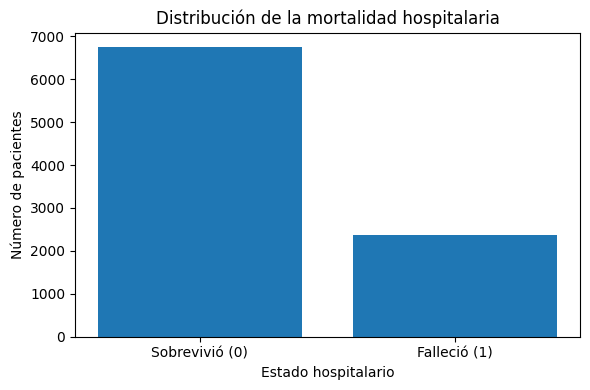
\includegraphics[width=\columnwidth]{figures/image7.png}
\caption{Distribución de la mortalidad hospitalaria.}
\label{fig:mortalidad}
\end{figure}
\FloatBarrier

Se obtuvieron 6745 pacientes sobrevivientes (74.08\,\%) y 2360 pacientes fallecidos (25.92\,\%). Este desbalance moderado implica que la exactitud global no representa adecuadamente el desempeño: un clasificador que siempre predice supervivencia alcanza un 74\,\% de accuracy sin detectar ningún fallecimiento. Por ello se emplean métricas complementarias como recall, precision, F1, ROC-AUC y Average Precision (Sección~\ref{sec:design}).

\subsection{Análisis de variables fisiológicas según mortalidad}
Con el objetivo de explorar posibles diferencias clínicas entre pacientes sobrevivientes y fallecidos, se analizaron las distribuciones de las principales variables fisiológicas disponibles en el dataset.

Se incluyeron presión arterial media (\texttt{meanbp}), frecuencia cardíaca (\texttt{hrt}), frecuencia respiratoria (\texttt{resp}), temperatura (\texttt{temp}), razón PaO$_2$/FiO$_2$ (\texttt{pafi}), albúmina (\texttt{alb}), bilirrubina (\texttt{bili}), creatinina (\texttt{crea}), sodio (\texttt{sod}), pH, glucosa (\texttt{glucose}), BUN (\texttt{bun}), recuento de leucocitos (\texttt{wblc}) y producción urinaria (\texttt{urine}).

Para cada variable se calcularon la media, mediana y desviación estándar de forma independiente para pacientes con \texttt{hospdead = 0} y \texttt{hospdead = 1}. Adicionalmente, se utilizaron diagramas de caja para visualizar diferencias en las distribuciones de algunas variables clínicas representativas.

Este análisis es de carácter exploratorio y permite identificar características potencialmente asociadas con la mortalidad hospitalaria, sin asumir todavía que dichas diferencias impliquen una relación causal o una capacidad predictiva independiente.

\subsection{Análisis de correlación entre variables numéricas}
Se evaluó la asociación lineal entre las principales variables numéricas y la mortalidad hospitalaria mediante el coeficiente de correlación de Pearson. Para facilitar la interpretación, se analizaron específicamente las correlaciones de cada característica con la variable objetivo \texttt{hospdead}, ordenándolas según su magnitud absoluta.

Este análisis permite identificar qué variables presentan una mayor asociación lineal con el desenlace hospitalario. Sin embargo, una correlación baja no implica necesariamente una baja utilidad predictiva, ya que pueden existir relaciones no lineales que posteriormente sean identificadas por los modelos de Machine Learning.

\begin{figure}[!t]
\centering
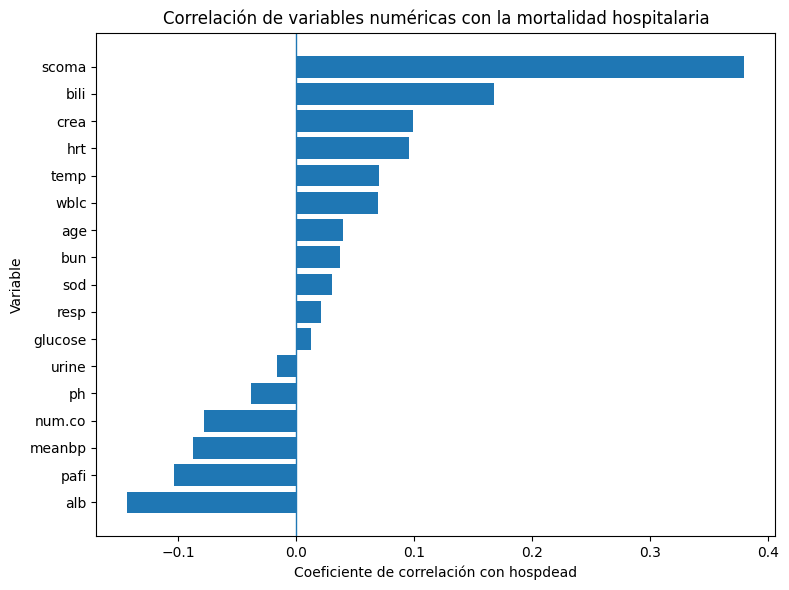
\includegraphics[width=\columnwidth]{figures/image2.png}
\caption{Correlación de variables numéricas con la mortalidad hospitalaria.}
\label{fig:correlacion}
\end{figure}

\FloatBarrier

\subsection{Identificación de valores atípicos}

\begin{figure}[!t]
\centering
\subfloat[Distribución de \texttt{meanbp} según mortalidad hospitalaria.\label{fig:meanbp}]{%
  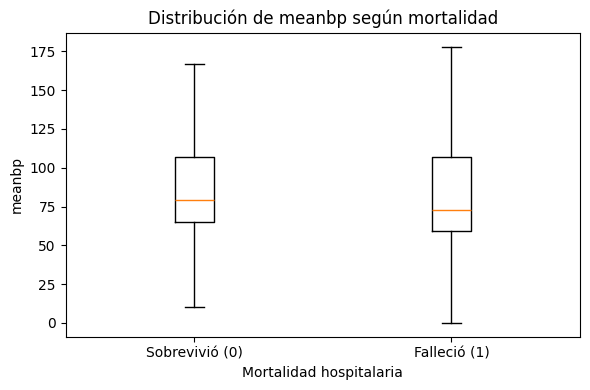
\includegraphics[width=\columnwidth]{figures/image3.png}%
}\\
\subfloat[Distribución de \texttt{hrt} según mortalidad hospitalaria.\label{fig:hrt}]{%
  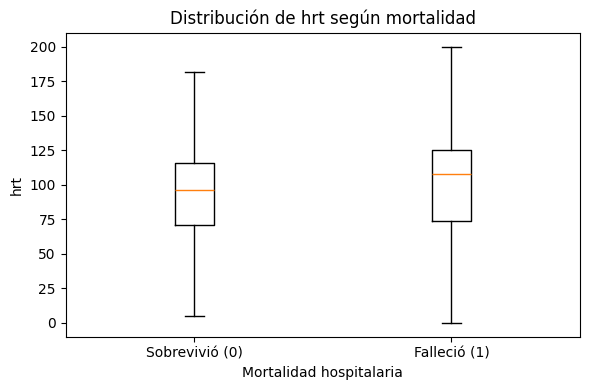
\includegraphics[width=\columnwidth]{figures/image4.png}%
}\\
\subfloat[Distribución de \texttt{resp} según mortalidad hospitalaria.\label{fig:resp}]{%
  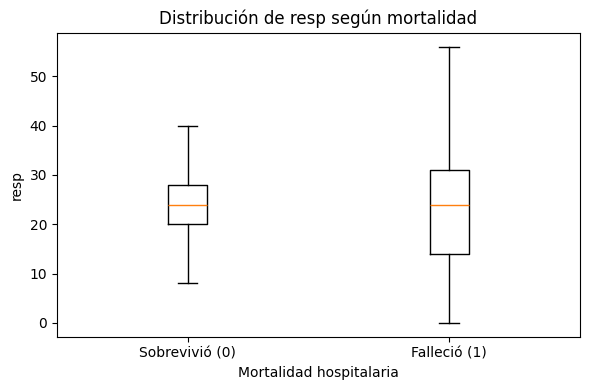
\includegraphics[width=\columnwidth]{figures/image8.png}%
}
\caption{Distribuciones de variables clínicas según mortalidad hospitalaria (1/2).}
\label{fig:dist_clinicas_a}
\end{figure}

\begin{figure}[!t]
\centering
\subfloat[Distribución de \texttt{crea} según mortalidad hospitalaria.\label{fig:crea}]{%
  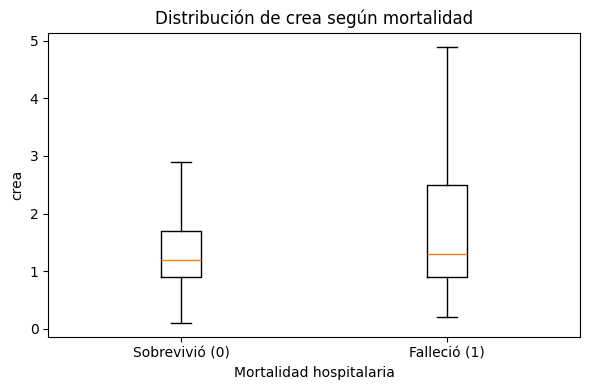
\includegraphics[width=\columnwidth]{figures/image6.png}%
}\\
\subfloat[Distribución de \texttt{bili} según mortalidad hospitalaria.\label{fig:bili}]{%
  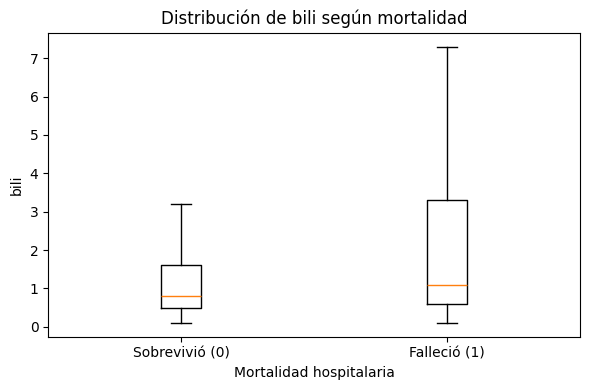
\includegraphics[width=\columnwidth]{figures/image5.png}%
}\\
\subfloat[Distribución de \texttt{alb} según mortalidad hospitalaria.\label{fig:alb}]{%
  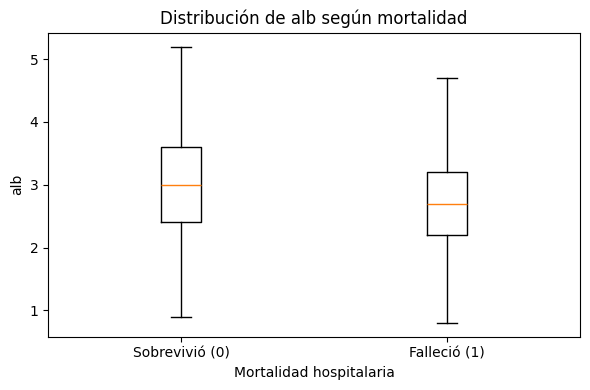
\includegraphics[width=\columnwidth]{figures/image1.png}%
}
\caption{Distribuciones de variables clínicas según mortalidad hospitalaria (2/2).}
\label{fig:dist_clinicas_b}
\end{figure}

Se evaluó la presencia de valores atípicos en las principales variables fisiológicas mediante el criterio del rango intercuartílico (IQR). Para cada variable se calcularon el primer cuartil (Q1), tercer cuartil (Q3) y el rango intercuartílico, definiendo como potenciales valores atípicos aquellas observaciones inferiores a $Q1 - 1.5\cdot IQR$ o superiores a $Q3 + 1.5\cdot IQR$.

Se calculó tanto el número como el porcentaje de observaciones identificadas como atípicas para cada variable. Sin embargo, estos valores no fueron eliminados. Debido a que el dataset corresponde a pacientes con enfermedades graves, mediciones fisiológicas extremas pueden representar condiciones clínicas reales y no necesariamente errores de registro.

\FloatBarrier
\subsection{Auditoría temporal}
Las evaluaciones clínicas corresponden al tercer día \emph{del estudio}, que no necesariamente coincide con el tercer día de hospitalización: 3157 pacientes ingresaron al estudio después de su primer día en el hospital (\texttt{hday} $>1$). Además, 138 fallecidos tienen \texttt{slos} $=3$ y \texttt{d.time} $=3$, es decir, sus mediciones pueden estar muy próximas al desenlace. Por ello, el experimento se interpreta como una clasificación retrospectiva y no como una validación clínica prospectiva.

\section{Preprocesamiento e ingeniería de características}
\label{sec:prepro}

\subsection{Partición y selección de variables}
Antes de cualquier transformación, los datos se dividieron de forma estratificada en entrenamiento (80\,\%, 7284 pacientes) y prueba (20\,\%, 1821 pacientes, 472 fallecidos) con semilla 42. La prevalencia es idéntica en ambas particiones (25.92\,\%). Dividir primero evita que estadísticos del conjunto de prueba (medianas, modas, medias o desviaciones) contaminen el entrenamiento.

Además de las 17 variables excluidas por fuga, se descartaron \texttt{adlp} y \texttt{urine} por superar el 50\,\% de valores faltantes en entrenamiento. Quedaron 27 predictores (21 numéricos y 6 categóricos), organizados en tres grupos para responder la pregunta de investigación:
\begin{itemize}
\item \textit{Demográficas (5):} \texttt{age}, \texttt{sex}, \texttt{race}, \texttt{income}, \texttt{edu}.
\item \textit{Clínicas (8):} \texttt{dzgroup}, \texttt{dzclass}, \texttt{num.co}, \texttt{diabetes}, \texttt{dementia}, \texttt{ca}, \texttt{adls}, \texttt{hday}.
\item \textit{Fisiológicas, día 3 (14):} \texttt{scoma}, \texttt{meanbp}, \texttt{wblc}, \texttt{hrt}, \texttt{resp}, \texttt{temp}, \texttt{pafi}, \texttt{alb}, \texttt{bili}, \texttt{crea}, \texttt{sod}, \texttt{ph}, \texttt{glucose}, \texttt{bun}.
\end{itemize}

\subsection{Transformaciones}
Todas las transformaciones forman parte de un \texttt{Pipeline} de scikit-learn \cite{pedregosa2011}, de modo que en cada fold de validación cruzada se reajustan solo con los datos de entrenamiento de ese fold:
\begin{itemize}
\item \textit{Numéricas:} imputación por la mediana, robusta frente a los valores extremos clínicamente plausibles que se decidió conservar. Opcionalmente se añaden indicadores binarios de valor faltante; su uso es un hiperparámetro elegido por validación cruzada, ya que en SUPPORT un laboratorio ausente suele indicar que no se solicitó.
\item \textit{Categóricas:} imputación por la moda y codificación \textit{one-hot}; las categorías no vistas en entrenamiento se ignoran.
\item \textit{Escalamiento:} estandarización $x'_j=(x_j-\mu_j)/\sigma_j$ solo para la regresión logística, porque la penalización $\lambda\lVert w\rVert$ depende de la escala de cada variable; los árboles son invariantes a transformaciones monótonas.
\end{itemize}

\subsection{Comparación de estrategias de imputación}
Se compararon cuatro estrategias para las variables numéricas, manteniendo fijos los hiperparámetros seleccionados: (i) mediana; (ii) valores ``normales'' recomendados por la documentación de SUPPORT (albúmina 3.5, PaO$_2$/FiO$_2$ 333.3, bilirrubina 1.01, creatinina 1.01, BUN 6.51, leucocitos 9) \cite{supportdata}, con mediana para el resto; (iii) KNN con $k=10$; e (iv) imputación iterativa tipo MICE. KNN e iterativa se aplican tras estandarizar. Se fijó de antemano la regla de abandonar la mediana solo si otra estrategia mejora el ROC-AUC de validación cruzada en más de 0.005 y en más de dos errores estándar de la diferencia pareada por fold.

\begin{table}[!t]
\centering
\footnotesize
\caption{ROC-AUC medio en CV (5 folds, entrenamiento) según la imputación numérica, con los hiperparámetros ya seleccionados. En negrita, el máximo por modelo.}
\label{tab:imputation}
\setlength{\tabcolsep}{4pt}
\begin{tabular}{lcccc}
\toprule
Modelo & Mediana & Normales & KNN & Iterativa \\
\midrule
Reg. logística & 0.804 & 0.804 & \textbf{0.805} & 0.804 \\
Árbol de decisión & 0.781 & 0.779 & \textbf{0.781} & 0.775 \\
Random Forest & 0.818 & \textbf{0.820} & 0.818 & 0.818 \\
Gradient Boosting & 0.823 & \textbf{0.826} & 0.824 & 0.822 \\
\bottomrule
\end{tabular}
\end{table}


Las diferencias fueron muy pequeñas (Tabla~\ref{tab:imputation}). La mayor mejora fue la de los valores normales en Gradient Boosting ($+0.0023$), por debajo del umbral fijado, por lo que se conservó la mediana en todos los modelos. Esto indica que el desempeño es robusto a la estrategia de imputación y que la información relevante del faltante se captura con los indicadores binarios.

\section{Metodología y modelos}
\label{sec:models}

\subsection{Baselines}
Se usaron dos referencias: (i) un \texttt{DummyClassifier} que predice la probabilidad previa $\hat P(y=1)$ para todos los pacientes y define el piso de desempeño, y (ii) una regresión logística entrenada solo con las 5 variables demográficas, que es el baseline de la pregunta de investigación.

\subsection{Modelos}
\textit{Regresión logística regularizada.} Modela $p=P(y=1\mid x)=\sigma(w^Tx+b)$ con $\sigma(z)=1/(1+e^{-z})$ y minimiza la entropía cruzada binaria más una penalización:
\begin{equation}
J(w,b)=-\frac1n\sum_{i=1}^{n}\left[y_i\ln p_i+(1-y_i)\ln(1-p_i)\right]+\lambda\,\Omega(w),
\end{equation}
con $\Omega(w)=\lVert w\rVert_2^2$ (ridge) o $\lVert w\rVert_1$ (lasso) y $C=1/\lambda$. Es el modelo interpretable de referencia: $e^{w_j}$ es el cambio multiplicativo en los odds por unidad de $x_j$.

\textit{Árbol de decisión (CART).} Particiona recursivamente con reglas $x_j\le t$ que maximizan la reducción de impureza (Gini $1-\sum_k\hat p_{mk}^2$ o entropía), y se poda por complejidad de costo $R_\alpha(T)=R(T)+\alpha\lvert T\rvert$. Es interpretable pero de alta varianza.

\textit{Random Forest} \cite{breiman2001}. Promedia $B=500$ árboles entrenados con muestras bootstrap y submuestreo aleatorio de variables en cada partición: $\bar p(x)=\frac1B\sum_b P_b(y=1\mid x)$. Reduce la varianza del árbol individual.

\textit{Gradient Boosting} \cite{friedman2001}. Construye un modelo aditivo $F_t(x)=F_{t-1}(x)+\eta\,h_t(x)$, donde cada árbol $h_t$ se ajusta al gradiente negativo de la log-loss. Reduce el sesgo de forma secuencial y captura no linealidades e interacciones. Se usó la implementación basada en histogramas de scikit-learn.

Se eligieron estos modelos para contrastar un modelo lineal interpretable con modelos no lineales de complejidad creciente y con las dos estrategias de ensamble vistas en el curso (bagging y boosting). La Tabla~\ref{tab:hparams} resume los espacios de búsqueda y los hiperparámetros seleccionados.

\begin{table*}[!tp]
\centering
\footnotesize
\caption{Hiperparámetros explorados con \texttt{RandomizedSearchCV} y valores seleccionados por ROC-AUC en validación cruzada.}
\label{tab:hparams}
\setlength{\tabcolsep}{4pt}
\begin{tabular}{lp{5.2cm}p{6.6cm}c}
\toprule
Modelo & Espacio de búsqueda & Seleccionado (CV) & Ind. faltantes \\
\midrule
Reg. logística & $C\in[10^{-3},10^{2}]$, L1/L2, \texttt{class\_weight} & L1, $C$=1.15, balanced & sí \\
Árbol de decisión & criterio, profundidad, hoja mín., $\alpha$ de poda & gini, prof.=8, hoja=77, $\alpha$=1.4e-05 & no \\
Random Forest & \texttt{max\_features}, profundidad, hoja mín., pesos & feat.=0.3, prof.=ninguno, hoja=20, balanced\_subsample & sí \\
Gradient Boosting & $\eta$, iteraciones, hojas, hoja mín., L2 & $\eta$=0.024, iter.=233, hojas=35, L2=1.25 & sí \\
\bottomrule
\end{tabular}
\end{table*}


\section{Diseño experimental y evaluación}
\label{sec:design}

\subsection{Estrategia de entrenamiento, validación y prueba}
La selección de hiperparámetros se realizó con \texttt{RandomizedSearchCV} (20 a 40 candidatos por modelo) y validación cruzada estratificada de $K=5$ folds, exclusivamente sobre el conjunto de entrenamiento:
\begin{equation}
CV(M,\theta)=\frac1K\sum_{k=1}^{K}\mathrm{Score}_k(M,\theta).
\end{equation}
El modelo final se eligió por el mayor ROC-AUC medio en validación cruzada. El conjunto de prueba se utilizó una sola vez, al final, para reportar métricas; no intervino en la selección de hiperparámetros, umbrales ni métodos de calibración.

\subsection{Métricas}
Con TP, FP, TN y FN definidos para la clase positiva (fallecimiento), se reportan accuracy $=(TP+TN)/N$, precision $=TP/(TP+FP)$, recall $=TP/(TP+FN)$, especificidad $=TN/(TN+FP)$ y $F_1=2PR/(P+R)$. Como métricas independientes del umbral se usan el ROC-AUC (métrica de selección, insensible a la prevalencia) y la Average Precision (AP, área bajo la curva precision-recall, más informativa con clases desbalanceadas; su valor de referencia es la prevalencia, 0.259). La calidad de las probabilidades se mide con el Brier score $\frac1n\sum_i(p_i-y_i)^2$, la log-loss y el error de calibración esperado $\mathrm{ECE}=\sum_b\frac{n_b}{N}\lvert\bar p_b-\bar y_b\rvert$ con 10 intervalos. Los intervalos de confianza de 95\,\% se obtienen con bootstrap percentil (1000 réplicas) sobre el conjunto de prueba, y las comparaciones entre modelos con diferencias pareadas sobre las mismas réplicas \cite{efron1993}.

\subsection{Umbral de decisión}
La predicción binaria es $\hat y=\mathbf 1[p\ge\tau]$. Como $\tau=0.5$ no es un umbral clínicamente validado, se elige $\tau$ maximizando F1 sobre predicciones \textit{out-of-fold} (OOF) del conjunto de entrenamiento. Adicionalmente se estudian (Sección~\ref{sec:thresholds}) un umbral con costos explícitos y umbrales por grupo diagnóstico.

\section{Resultados y análisis}

\subsection{Selección de modelos}
La Tabla~\ref{tab:cv} muestra los resultados de validación cruzada. Gradient Boosting obtuvo el mayor ROC-AUC (0.823 $\pm$ 0.008), seguido de Random Forest (0.818). La brecha entre el AUC de entrenamiento y el de validación es mayor en los ensambles (0.12 en Gradient Boosting) que en la regresión logística (0.01), lo que refleja su mayor varianza; aun así, generalizan mejor.

\begin{table}[!t]
\centering
\footnotesize
\caption{Validación cruzada estratificada (5 folds, solo entrenamiento) del mejor candidato de cada modelo. En negrita, el modelo seleccionado.}
\label{tab:cv}
\setlength{\tabcolsep}{4pt}
\begin{tabular}{lcccc}
\toprule
Modelo & AUC train & AUC CV & AP CV & Log-loss CV \\
\midrule
Dummy (prior) & 0.500 & 0.500 $\pm$ 0.000 & 0.259 & 0.572 \\
Reg. logística & 0.814 & 0.804 $\pm$ 0.007 & 0.609 & 0.537 \\
Árbol de decisión & 0.819 & 0.781 $\pm$ 0.012 & 0.558 & 0.474 \\
Random Forest & 0.904 & 0.818 $\pm$ 0.010 & 0.627 & 0.495 \\
\textbf{Gradient Boosting} & 0.947 & 0.823 $\pm$ 0.008 & 0.646 & 0.432 \\
\bottomrule
\end{tabular}
\end{table}


La curva de validación del árbol sin poda (Fig.~\ref{fig:valcurve}) ilustra el compromiso sesgo-varianza: el AUC de validación alcanza su máximo con profundidad 5 (0.774), mientras que con profundidad 20 el AUC de entrenamiento llega a 0.999 y el de validación cae a 0.609.

\begin{figure}[!t]
\centering
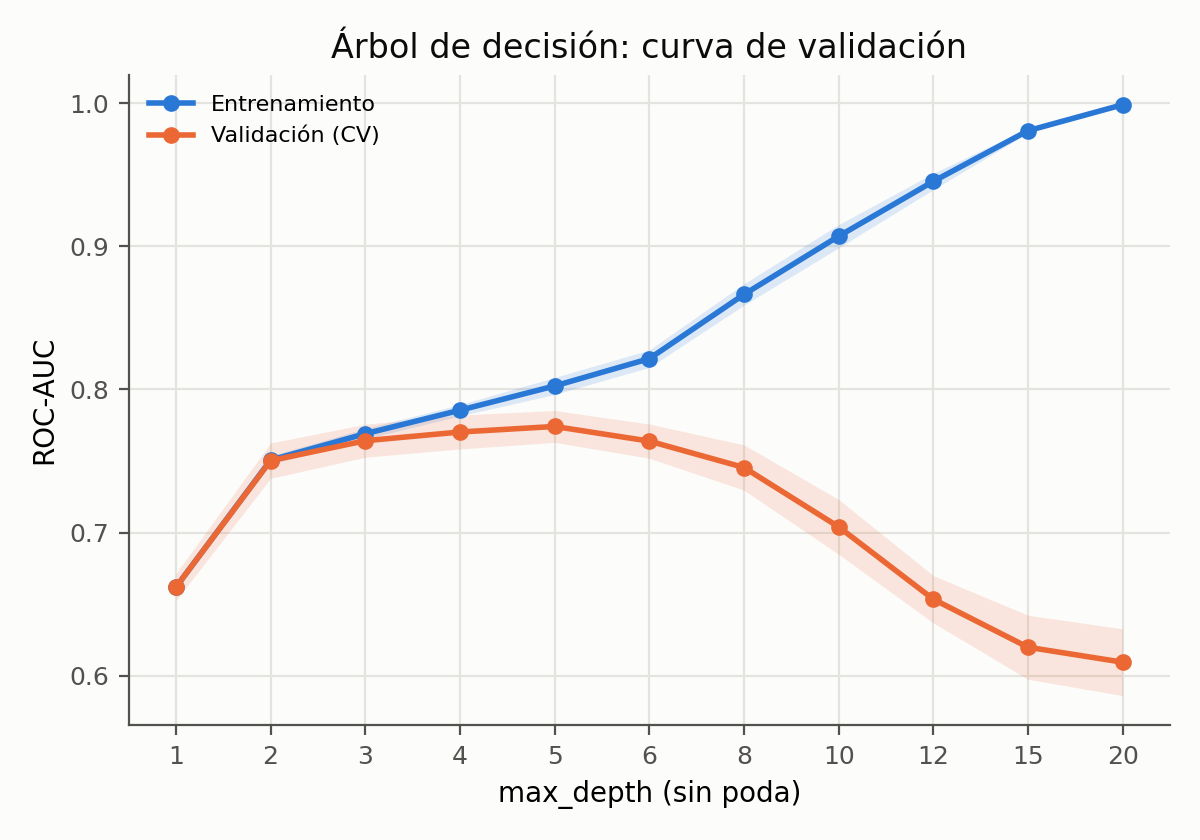
\includegraphics[width=0.9\columnwidth]{figures/p2_tree_validation_curve.png}
\caption{Curva de validación del árbol de decisión sin poda (ROC-AUC, media $\pm$ 1 DE en 5 folds).}
\label{fig:valcurve}
\end{figure}

\subsection{Desempeño en prueba}
La Tabla~\ref{tab:test} y la Fig.~\ref{fig:rocpr} presentan los resultados en prueba. Todos los modelos superan ampliamente al baseline. Gradient Boosting obtuvo un ROC-AUC de 0.834 y un AP de 0.655; con $\tau=0.29$ detecta el 70.3\,\% de los fallecimientos (recall) con una precision de 0.535. Su AUC en prueba es coherente con el de validación cruzada (0.823), por lo que no hay indicios de sobreajuste al proceso de selección.

\begin{table*}[!tp]
\centering
\scriptsize
\caption{Resultados en el conjunto de prueba ($n=1821$, 472 fallecidos). $\tau$ se eligió maximizando F1 en predicciones \textit{out-of-fold} de entrenamiento (0.5 para el Dummy). IC por bootstrap (1000 réplicas).}
\label{tab:test}
\setlength{\tabcolsep}{4pt}
\begin{tabular}{lcccccccccc}
\toprule
Modelo & $\tau$ & Acc. & Prec. & Recall & Espec. & F1 & ROC-AUC [IC 95\%] & AP [IC 95\%] & Brier & TP/FP/FN/TN \\
\midrule
Dummy (prior) & 0.50 & 0.741 & 0.000 & 0.000 & 1.000 & 0.000 & 0.500 & 0.259 & 0.192 & 0/0/472/1349 \\
Reg. logística & 0.53 & 0.767 & 0.539 & 0.695 & 0.792 & 0.607 & 0.820 [0.800, 0.842] & 0.629 [0.583, 0.675] & 0.171 & 328/280/144/1069 \\
Árbol de decisión & 0.31 & 0.753 & 0.518 & 0.661 & 0.785 & 0.581 & 0.799 [0.778, 0.821] & 0.575 [0.527, 0.626] & 0.149 & 312/290/160/1059 \\
Random Forest & 0.54 & 0.778 & 0.559 & 0.674 & 0.814 & 0.611 & 0.832 [0.813, 0.853] & 0.641 [0.595, 0.688] & 0.160 & 318/251/154/1098 \\
\textbf{Gradient Boosting} & 0.29 & 0.765 & 0.535 & 0.703 & 0.787 & 0.608 & 0.834 [0.814, 0.854] & 0.655 [0.611, 0.700] & 0.136 & 332/288/140/1061 \\
\bottomrule
\end{tabular}
\end{table*}


\begin{figure*}[!tp]
\centering
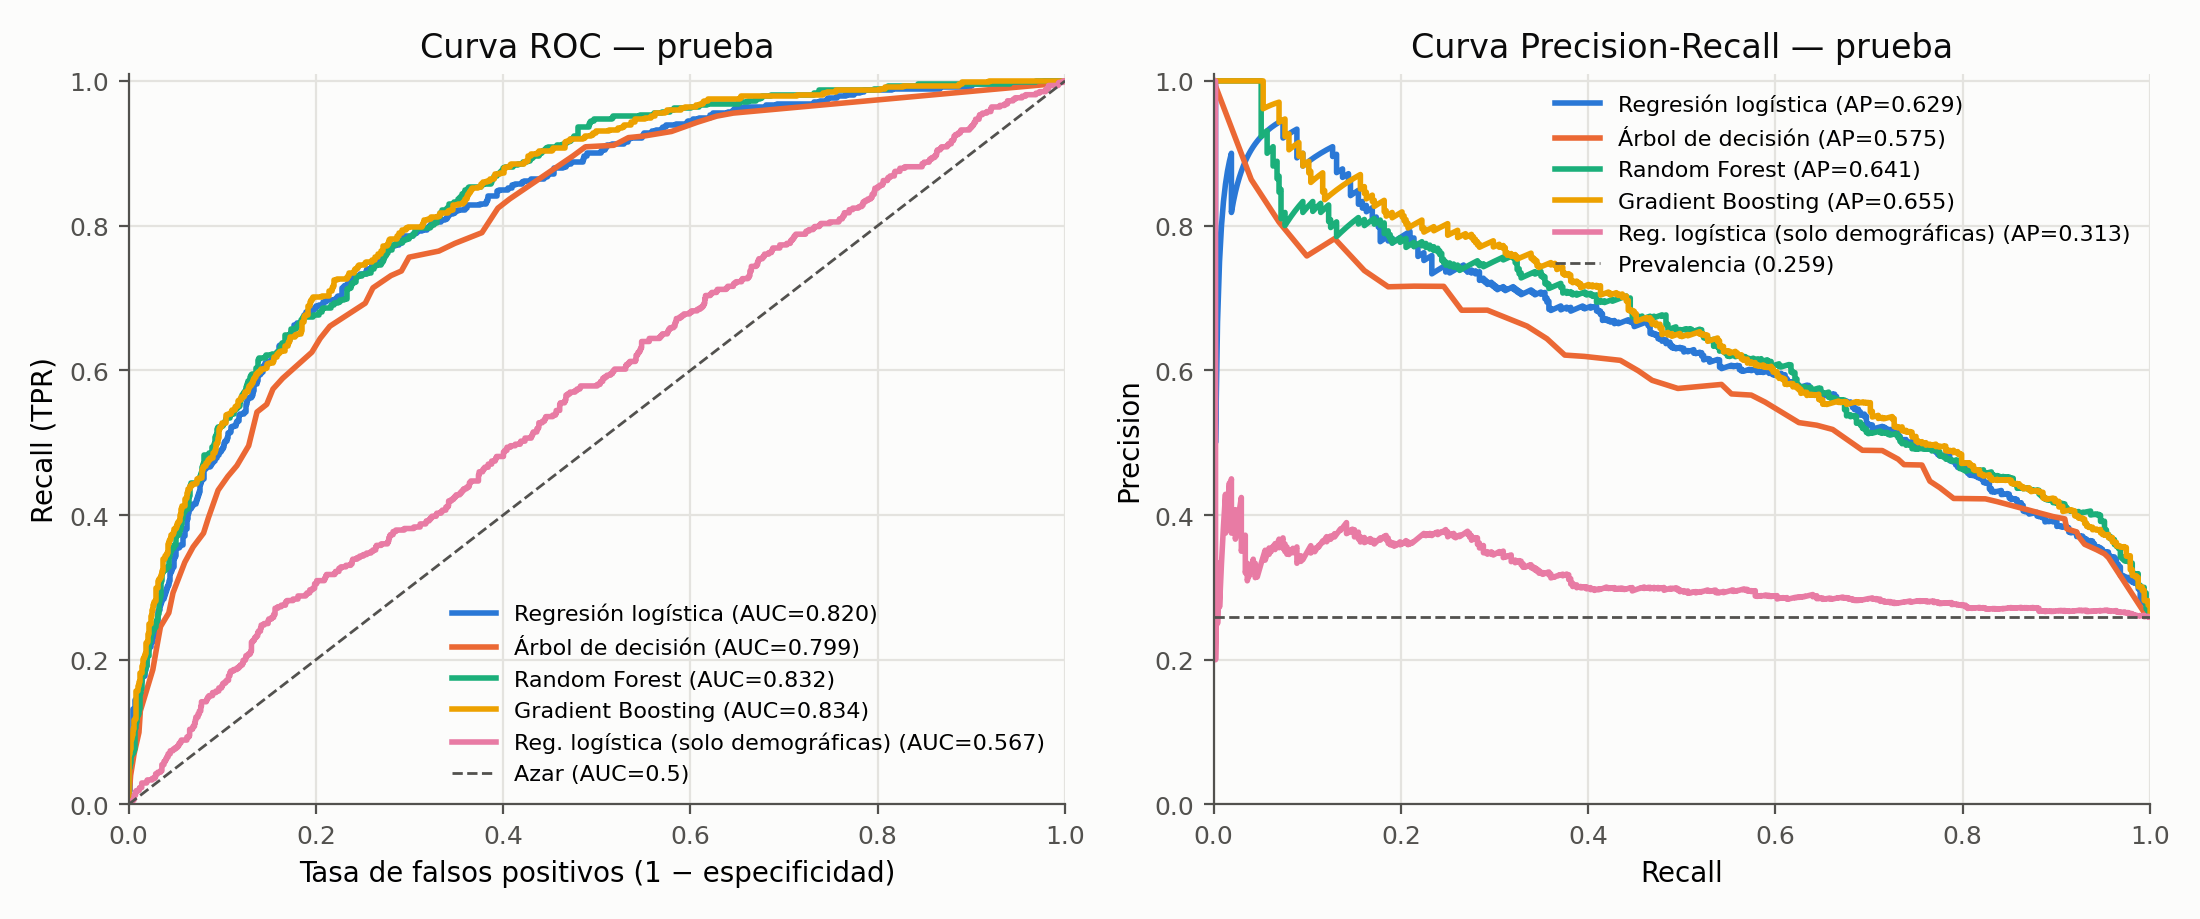
\includegraphics[width=0.85\textwidth]{figures/p2_roc_pr_curves.png}
\caption{Curvas ROC y precision-recall en prueba. La línea discontinua del panel derecho indica la prevalencia (AP de un clasificador aleatorio).}
\label{fig:rocpr}
\end{figure*}

\begin{figure*}[!tp]
\centering
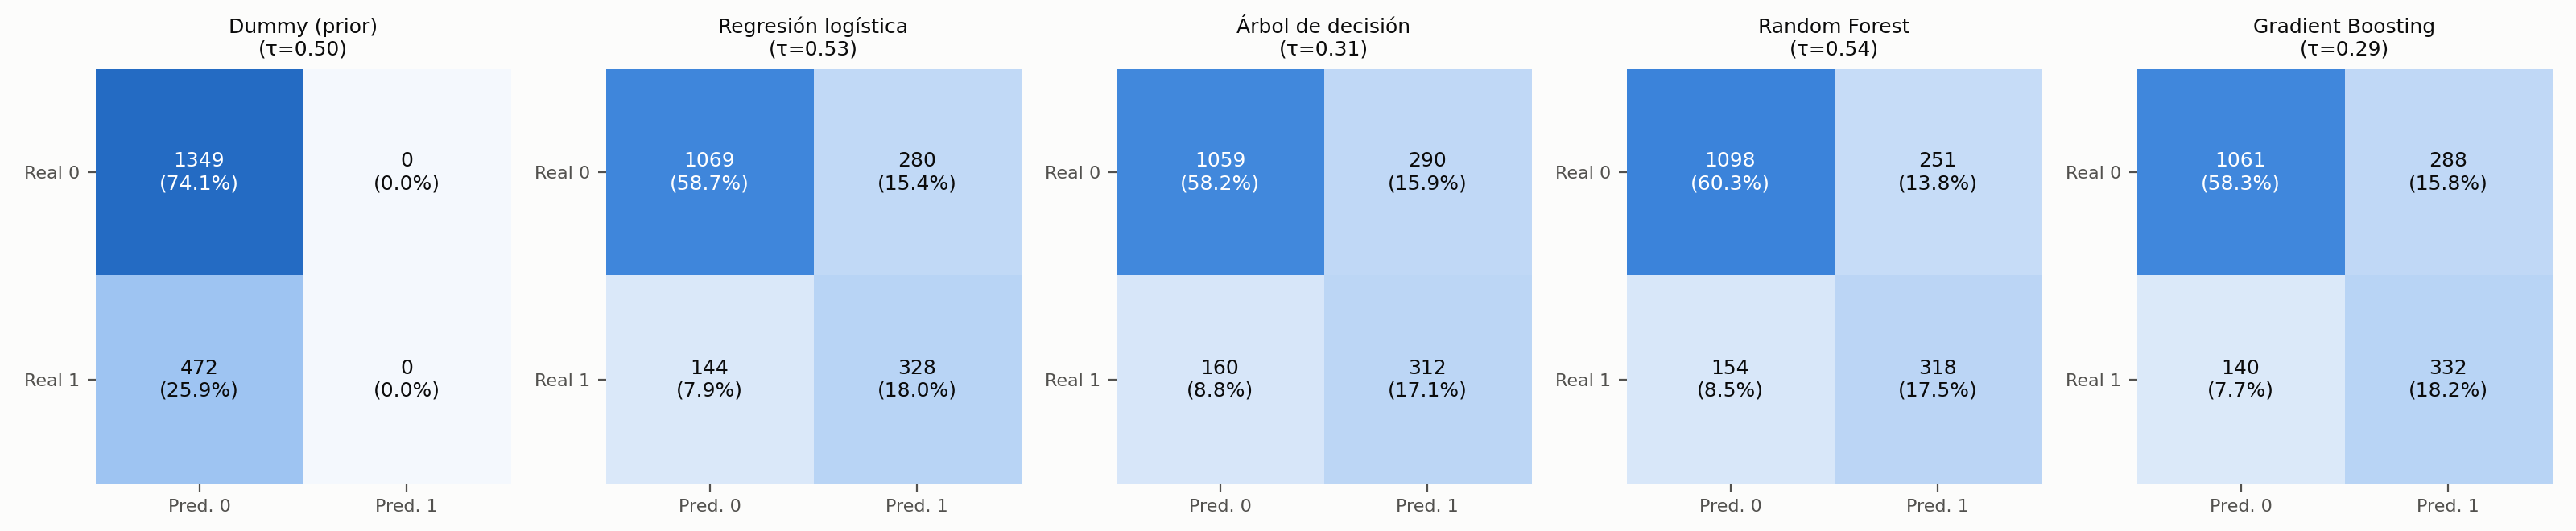
\includegraphics[width=\textwidth]{figures/p2_confusion_matrices.png}
\caption{Matrices de confusión en prueba con el umbral $\tau$ elegido en validación cruzada (filas: clase real; columnas: clase predicha).}
\label{fig:confusion}
\end{figure*}

Las diferencias pareadas de ROC-AUC frente a Gradient Boosting fueron $-0.002$ (IC 95\,\%: $-0.008$ a $0.004$) para Random Forest, $-0.015$ ($-0.024$ a $-0.005$) para la regresión logística y $-0.035$ ($-0.049$ a $-0.020$) para el árbol. Por lo tanto, los dos ensambles son estadísticamente indistinguibles, mientras que ambos superan a la regresión logística por un margen pequeño y al árbol individual por un margen mayor. Con el umbral por defecto $\tau=0.5$, Gradient Boosting alcanza una accuracy de 0.804, pero un recall de solo 0.443: deja sin detectar más de la mitad de los fallecimientos, lo que justifica elegir el umbral explícitamente.

\subsection{Pregunta de investigación: variables fisiológicas frente a demográficas}
Se repitió la búsqueda completa de hiperparámetros con tres conjuntos de variables (Tabla~\ref{tab:ablation}). Con solo variables demográficas, ambos modelos apenas superan el azar (ROC-AUC $\approx$ 0.57 en prueba). Añadir las 14 variables fisiológicas eleva el AUC de la regresión logística en $+0.192$ (IC 95\,\%: 0.161 a 0.227) y el de Gradient Boosting en $+0.227$. Las variables clínicas (diagnóstico, comorbilidades y estado funcional) aportan un incremento adicional menor, de $+0.04$ a $+0.06$.

\begin{table}[!t]
\centering
\scriptsize
\caption{ROC-AUC por conjunto de variables (RL: regresión logística; GB: Gradient Boosting). $\Delta$AUC RL: diferencia pareada en prueba frente a la RL solo demográfica [IC 95\,\%].}
\label{tab:ablation}
\setlength{\tabcolsep}{4pt}
\begin{tabular}{lccccc}
\toprule
Variables & RL CV & RL test & GB CV & GB test & $\Delta$AUC RL \\
\midrule
Demog. & 0.570 & 0.567 & 0.575 & 0.569 & --- \\
Demog.+fisiol. & 0.751 & 0.758 & 0.785 & 0.796 & +0.192 [0.16, 0.23] \\
Todas & 0.804 & 0.820 & 0.823 & 0.834 & +0.254 [0.22, 0.29] \\
\bottomrule
\end{tabular}
\end{table}


Con solo variables demográficas, Gradient Boosting no mejora a la regresión logística (diferencia de AUC $+0.002$, IC 95\,\%: $-0.019$ a $0.024$). En cambio, con variables fisiológicas sí la supera (0.796 frente a 0.758): la relación entre la fisiología y la mortalidad es no lineal, por ejemplo con riesgo elevado en ambos extremos de la presión arterial o la temperatura.

\subsection{Interpretación}
La importancia por permutación del modelo final (Fig.~\ref{fig:importance}) mide la caída del ROC-AUC en prueba al permutar cada variable. El predictor más importante es \texttt{scoma} (escala de coma; 0.073), seguido de \texttt{dzclass} (0.027), \texttt{hday} (0.024) y \texttt{age} (0.014). Sumadas por grupo, las variables fisiológicas acumulan 0.113, las clínicas 0.062 y las demográficas 0.017; \texttt{sex}, \texttt{income} y \texttt{race} tienen importancia prácticamente nula. Como la permutación reparte la importancia entre variables correlacionadas (por ejemplo, \texttt{dzgroup} y \texttt{dzclass}), la importancia individual de estas se subestima.

\begin{figure}[!t]
\centering
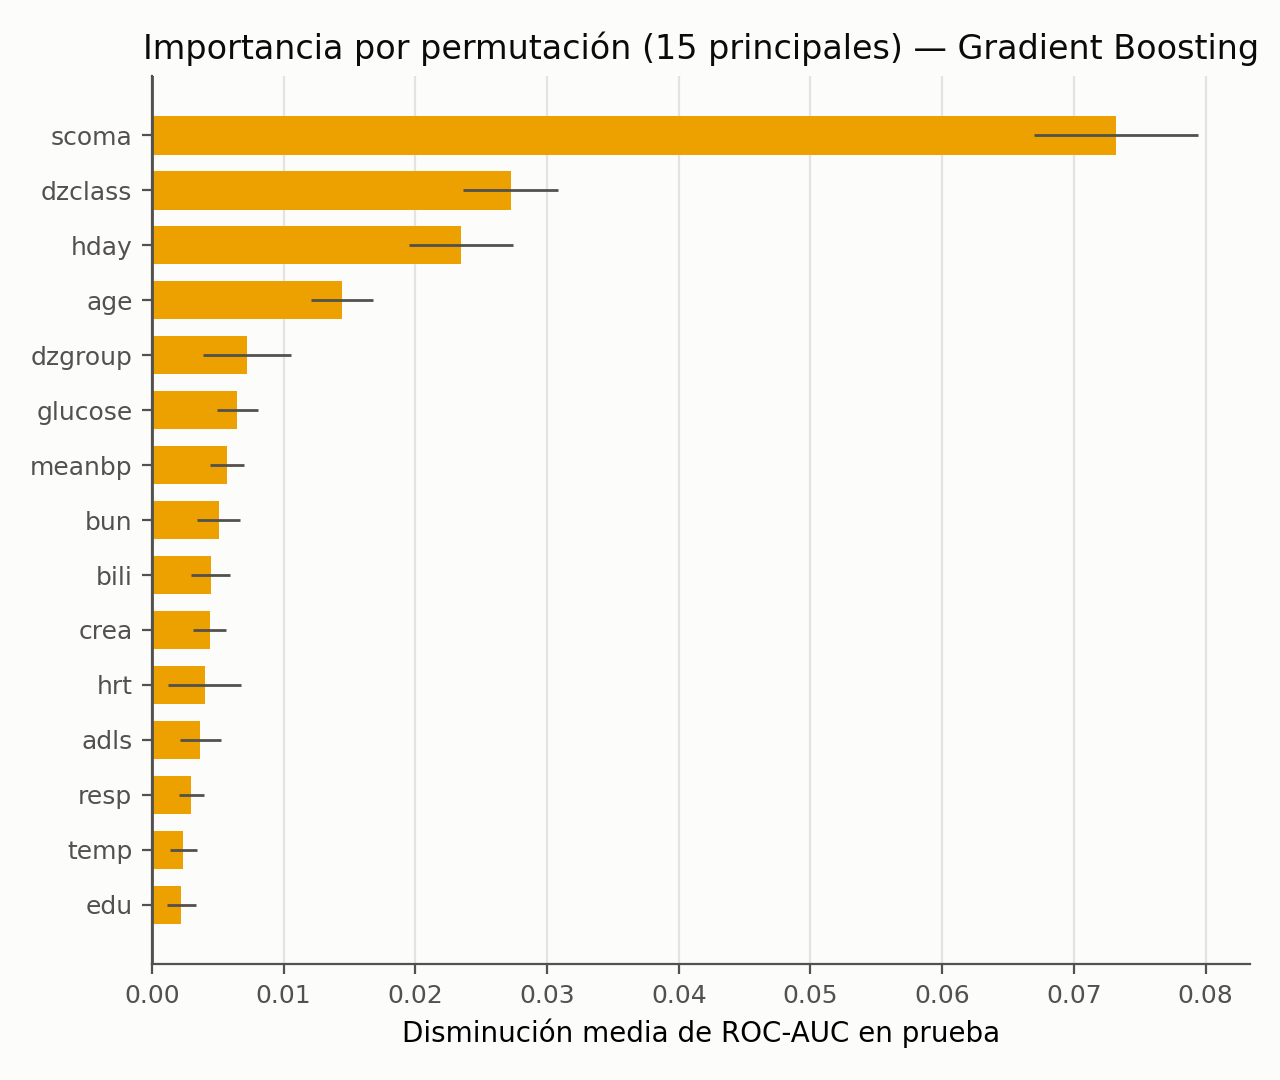
\includegraphics[width=0.85\columnwidth]{figures/p2_permutation_importance_top15.png}
\caption{Importancia por permutación (15 variables principales) del modelo final en prueba; barras: media y DE en 20 repeticiones.}
\label{fig:importance}
\end{figure}

En la regresión logística (lasso, $C=1.15$), los coeficientes de mayor magnitud corresponden al grupo diagnóstico (odds ratio 2.02 para falla multiorgánica con malignidad, 1.90 para cirrosis, 0.51 para insuficiencia cardíaca y 0.54 para cáncer de colon) y a \texttt{scoma} (OR 1.80 por desviación estándar). La penalización L1 anuló los coeficientes de \texttt{sex}=masculino, \texttt{race}=negra e \texttt{income}$>$\$50k. Estas son asociaciones predictivas condicionadas al resto de variables, no efectos causales.

\subsection{Calibración y recalibración}
La regresión logística y Random Forest seleccionaron \texttt{class\_weight="balanced"}, que repondera la clase minoritaria y desplaza las probabilidades hacia la clase positiva: ambos modelos sobrestiman sistemáticamente el riesgo (ECE de 0.166 y 0.140 en prueba). Para corregirlo se aplicó recalibración de Platt (sigmoide) \cite{platt1999} e isotónica \cite{zadrozny2002} mediante \texttt{CalibratedClassifierCV} con 5 folds dentro de entrenamiento, eligiendo el método por el menor Brier OOF (Tabla~\ref{tab:calibration}, Fig.~\ref{fig:recal}).

\begin{table*}[!tp]
\centering
\footnotesize
\caption{Recalibración con \texttt{CalibratedClassifierCV} (5 folds dentro de entrenamiento). $^{*}$Menor Brier \textit{out-of-fold} en entrenamiento; en Gradient Boosting no se adoptó (ver texto).}
\label{tab:calibration}
\setlength{\tabcolsep}{4pt}
\begin{tabular}{llccccc}
\toprule
Modelo & Calibración & Brier OOF & Brier test & ECE test & Log-loss test & AUC test \\
\midrule
Reg. logística & Sin recalibrar & 0.179 & 0.171 & 0.166 & 0.519 & 0.820 \\
 & Platt$^{*}$ & 0.146 & 0.141 & 0.024 & 0.438 & 0.820 \\
 & Isotónica & 0.146 & 0.142 & 0.020 & 0.439 & 0.818 \\
Random Forest & Sin recalibrar & 0.164 & 0.160 & 0.140 & 0.484 & 0.832 \\
 & Platt & 0.143 & 0.139 & 0.035 & 0.429 & 0.830 \\
 & Isotónica$^{*}$ & 0.142 & 0.139 & 0.026 & 0.428 & 0.830 \\
Gradient Boosting & Sin recalibrar & 0.140 & 0.136 & 0.020 & 0.422 & 0.834 \\
 & Platt$^{*}$ & 0.139 & 0.135 & 0.024 & 0.419 & 0.838 \\
 & Isotónica & 0.139 & 0.135 & 0.024 & 0.416 & 0.838 \\
\bottomrule
\end{tabular}
\end{table*}


La recalibración redujo el ECE en prueba de la regresión logística de 0.166 a 0.024 (Platt) y el de Random Forest de 0.140 a 0.026 (isotónica), y el Brier score de 0.171 a 0.141 y de 0.160 a 0.139, respectivamente, sin alterar su capacidad de discriminación (ROC-AUC prácticamente igual). Gradient Boosting, entrenado sin pesos de clase, ya estaba bien calibrado (ECE 0.020), y la recalibración solo produjo una mejora marginal (Brier 0.136 a 0.135).

\begin{figure*}[!tp]
\centering
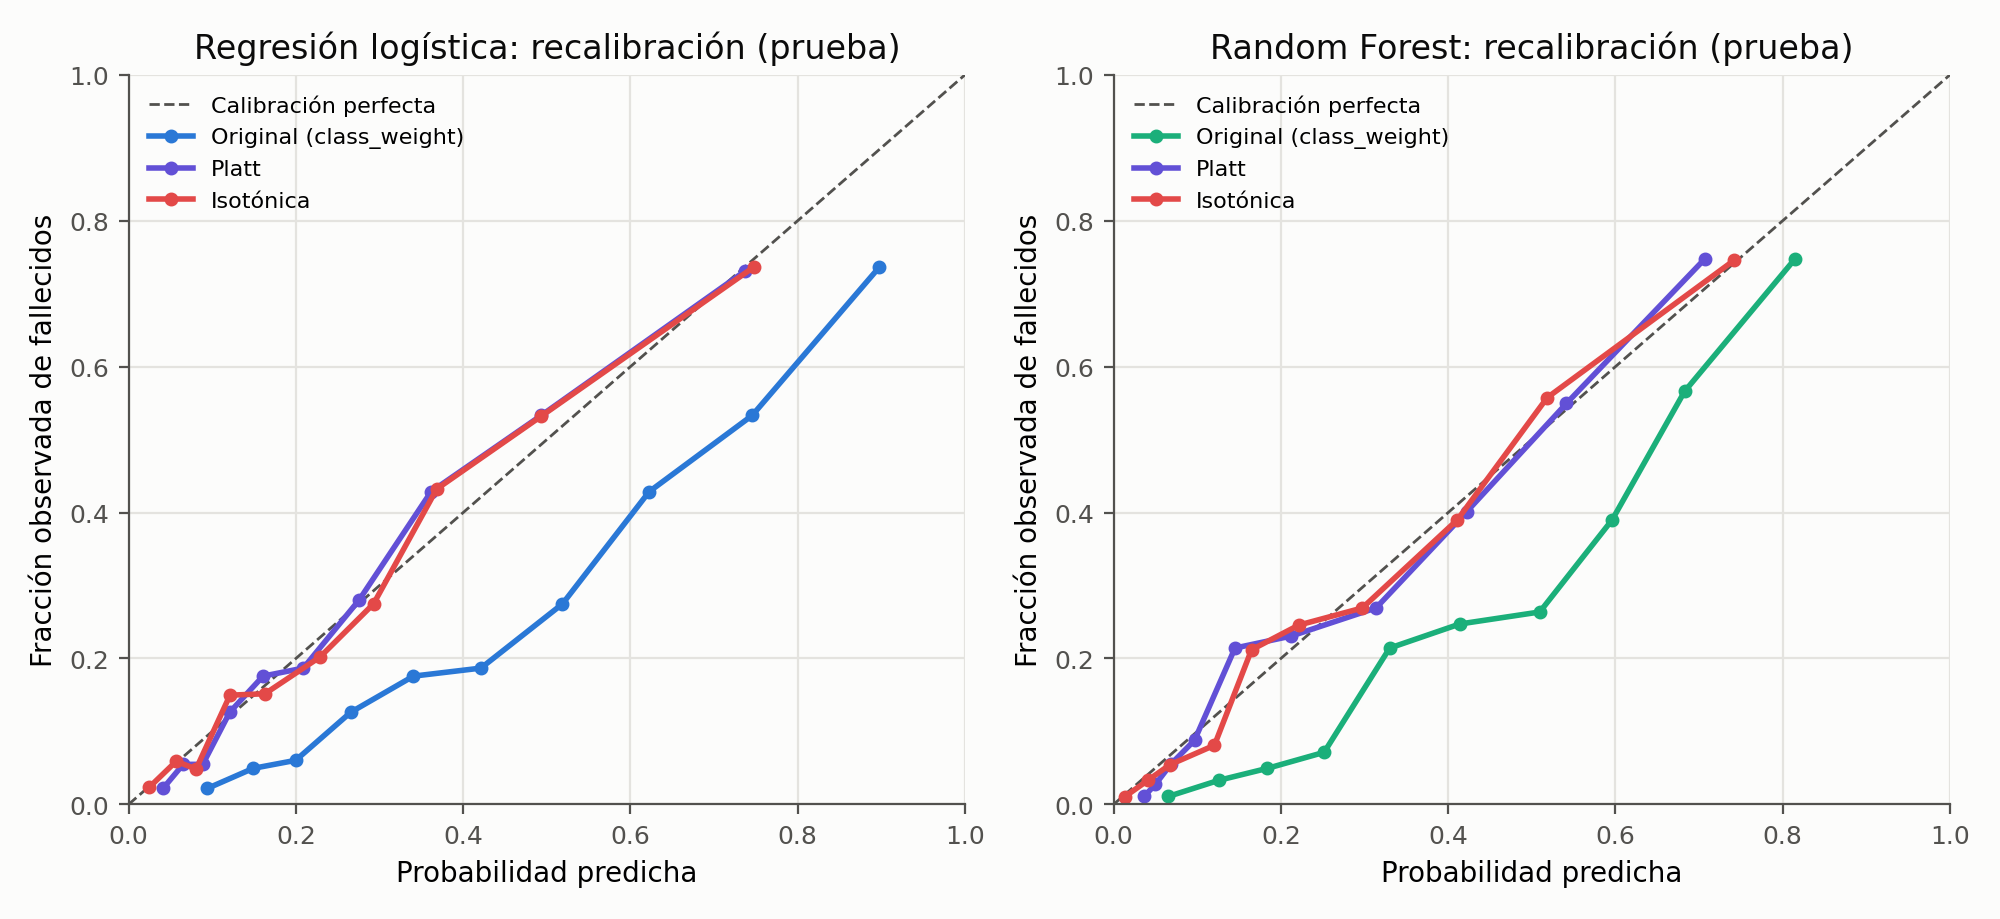
\includegraphics[width=0.8\textwidth]{figures/p2x_recalibration.png}
\caption{Curvas de calibración en prueba de los modelos con pesos de clase, antes y después de la recalibración.}
\label{fig:recal}
\end{figure*}

\subsection{Umbrales con costos clínicos y por grupo diagnóstico}
\label{sec:thresholds}
Asignando un costo $C_{FP}=1$ a una falsa alerta y $C_{FN}=R$ a un fallecimiento no detectado, la regla de Bayes con probabilidades calibradas da el umbral $\tau^*=C_{FP}/(C_{FP}+C_{FN})=1/(1+R)$ \cite{elkan2001}. Como no existe una razón de costos validada para esta población, se presenta un análisis de sensibilidad con $R\in\{1,2,3,5,10\}$, comparando $\tau^*$ con el umbral $\hat\tau$ que minimiza el costo en predicciones OOF de entrenamiento (Tabla~\ref{tab:costs}, Fig.~\ref{fig:costs}).

\begin{table*}[!tp]
\centering
\footnotesize
\caption{Umbral con costos explícitos ($C_{FP}=1$, $C_{FN}=R$) para el modelo final. $\tau^{*}=1/(1+R)$ (regla de Bayes); $\hat\tau$ minimiza el costo en predicciones OOF de entrenamiento. Métricas y costo medio por paciente en prueba (con $\hat\tau$). Costo trivial: mejor entre no alertar a nadie o alertar a todos.}
\label{tab:costs}
\setlength{\tabcolsep}{4pt}
\begin{tabular}{ccccccccc}
\toprule
$R$ & $\tau^{*}$ & $\hat\tau$ & Recall & Prec. & Espec. & Costo $\tau^{*}$ & Costo $\hat\tau$ & Costo trivial \\
\midrule
1 & 0.500 & 0.55 & 0.381 & 0.729 & 0.950 & 0.196 & 0.197 & 0.259 \\
2 & 0.333 & 0.30 & 0.701 & 0.547 & 0.797 & 0.315 & 0.305 & 0.518 \\
3 & 0.250 & 0.25 & 0.752 & 0.502 & 0.739 & 0.386 & 0.386 & 0.741 \\
5 & 0.167 & 0.16 & 0.886 & 0.431 & 0.591 & 0.459 & 0.451 & 0.741 \\
10 & 0.091 & 0.08 & 0.975 & 0.352 & 0.373 & 0.539 & 0.530 & 0.741 \\
\bottomrule
\end{tabular}
\end{table*}


Como Gradient Boosting está bien calibrado, $\tau^*$ y $\hat\tau$ prácticamente coinciden (por ejemplo, ambos valen 0.25 para $R=3$). El modelo tiene un costo menor que las estrategias triviales de no alertar a nadie o alertar a todos en todos los valores de $R$; para $R=3$, el costo medio por paciente es 0.386 frente a 0.741 de la mejor estrategia trivial. A medida que aumenta $R$, el umbral baja y el recall crece a costa de la especificidad: con $R=10$ ($\hat\tau=0.08$) se detecta el 97.5\,\% de los fallecimientos, pero la especificidad cae a 0.373.

\begin{figure}[!t]
\centering
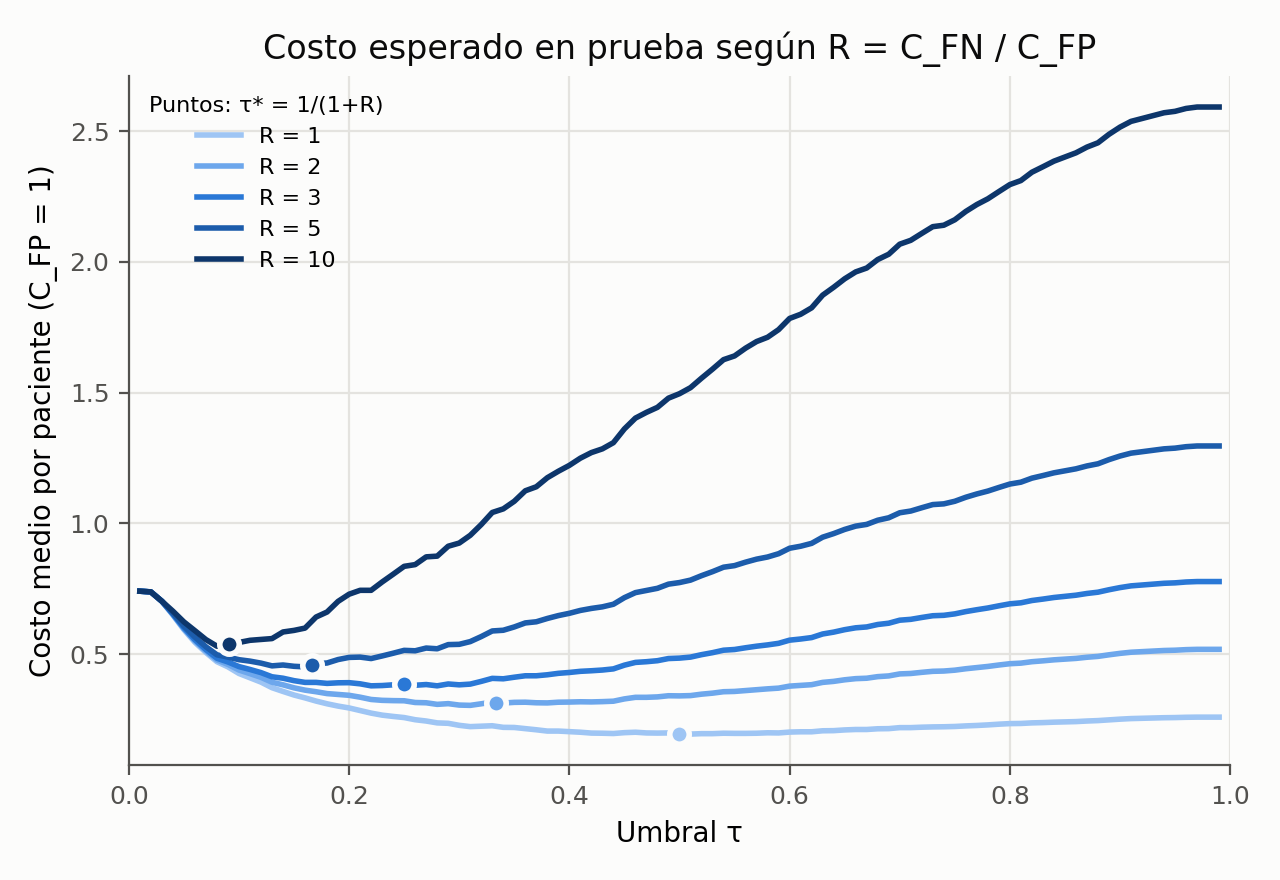
\includegraphics[width=0.8\columnwidth]{figures/p2x_cost_curves.png}
\caption{Costo medio por paciente en prueba según el umbral para distintas razones de costo $R$. Los puntos marcan $\tau^*=1/(1+R)$.}
\label{fig:costs}
\end{figure}

Por último, se comparó el umbral global con umbrales específicos por grupo diagnóstico, elegidos en predicciones OOF de entrenamiento (Tabla~\ref{tab:groups}). Con el umbral global, los errores se concentran por grupo: en insuficiencia cardíaca, EPOC y cáncer de pulmón, de baja mortalidad, se pierde cerca del 80\,\% de los fallecimientos (FNR 0.78--0.83), mientras que en falla multiorgánica con malignidad y coma, de alta mortalidad, se alerta a cerca del 80\,\% de los sobrevivientes (FPR 0.78--0.84). Los umbrales por grupo redistribuyen estos errores (por ejemplo, con criterio F1 el FNR en EPOC baja de 0.78 a 0.37 a cambio de un FPR de 0.22), pero no mejoran el desempeño global: el F1 pasó de 0.608 a 0.596 y el costo con $R=3$ quedó prácticamente igual (0.386). Esto es lo esperado con probabilidades calibradas, para las que el umbral óptimo por costo es el mismo en todos los grupos. Además, los umbrales por grupo son inestables en grupos pequeños (en EPOC, 0.13 con F1 frente a 0.37 con costo). La limitación de fondo es la baja discriminación \emph{dentro} de cada grupo (ROC-AUC de 0.69 a 0.81, salvo cáncer de colon, con solo 6 fallecidos en prueba), que no se corrige moviendo el umbral.

\begin{table*}[!tp]
\centering
\scriptsize
\caption{Umbral global frente a umbral por grupo diagnóstico (modelo final, prueba). Cada celda: $\tau$ / FNR / FPR. Última fila: recall, F1 y costo medio por paciente ($R$=3). Todos los umbrales se eligieron en predicciones OOF de entrenamiento.}
\label{tab:groups}
\setlength{\tabcolsep}{4pt}
\begin{tabular}{lrcccc}
\toprule
Grupo & $n$ & Global F1 & Por grupo F1 & Global costo $R$=3 & Por grupo costo $R$=3 \\
\midrule
ARF/MOSF w/Sepsis & 711 & 0.29 / 0.30 / 0.38 & 0.27 / 0.27 / 0.41 & 0.25 / 0.23 / 0.48 & 0.26 / 0.24 / 0.44 \\
CHF & 272 & 0.29 / 0.81 / 0.00 & 0.20 / 0.81 / 0.02 & 0.25 / 0.81 / 0.01 & 0.21 / 0.81 / 0.01 \\
COPD & 201 & 0.29 / 0.78 / 0.04 & 0.13 / 0.37 / 0.22 & 0.25 / 0.74 / 0.05 & 0.37 / 0.89 / 0.02 \\
Lung Cancer & 170 & 0.29 / 0.83 / 0.01 & 0.16 / 0.50 / 0.12 & 0.25 / 0.83 / 0.03 & 0.16 / 0.50 / 0.10 \\
MOSF w/Malig & 137 & 0.29 / 0.03 / 0.84 & 0.30 / 0.03 / 0.83 & 0.25 / 0.03 / 0.96 & 0.30 / 0.03 / 0.83 \\
Coma & 119 & 0.29 / 0.07 / 0.78 & 0.42 / 0.19 / 0.57 & 0.25 / 0.03 / 0.82 & 0.16 / 0.00 / 0.94 \\
Cirrhosis & 112 & 0.29 / 0.47 / 0.09 & 0.26 / 0.42 / 0.11 & 0.25 / 0.42 / 0.12 & 0.22 / 0.42 / 0.18 \\
Colon Cancer & 99 & 0.29 / 0.67 / 0.00 & 0.16 / 0.50 / 0.02 & 0.25 / 0.67 / 0.01 & 0.19 / 0.67 / 0.01 \\
\textit{Global} & 1821 & Rec 0.70 / F1 0.61 / C 0.389 & Rec 0.74 / F1 0.60 / C 0.395 & Rec 0.75 / F1 0.60 / C 0.386 & Rec 0.75 / F1 0.60 / C 0.386 \\
\bottomrule
\end{tabular}
\end{table*}


\subsection{Análisis de errores y subgrupos}
Con $\tau=0.29$, el modelo final produjo 332 verdaderos positivos, 140 falsos negativos, 288 falsos positivos y 1061 verdaderos negativos. Los falsos negativos son fallecidos que el día 3 parecían estables: mediana de \texttt{scoma} 0 frente a 37 en los verdaderos positivos, ingreso al estudio en el primer día de hospitalización (\texttt{hday} 1 frente a 5), frecuencia cardíaca de 90 frente a 110 y temperatura de 36.7 frente a 37.5\,$^{\circ}$C. Es decir, el modelo no puede anticipar deterioros posteriores a las mediciones disponibles. Los falsos positivos, en cambio, comparten el perfil de gravedad de los verdaderos positivos.

Por sexo, el ROC-AUC fue de 0.849 en mujeres y 0.825 en hombres (FNR 0.26 y 0.32), y por raza de 0.835 en pacientes blancos y 0.802 en pacientes negros (FNR 0.30 y 0.34). El desempeño fue estable entre grupos de edad (ROC-AUC 0.825--0.844). Los grupos de raza asiática ($n=17$) y otras ($n=14$) son demasiado pequeños para extraer conclusiones, y estas diferencias son descriptivas: no se evaluó su significancia estadística.

\section{Discusión y limitaciones}
\textit{?`Por qué funcionan mejor los ensambles?} Los ensambles de árboles capturan no linealidades (riesgo en ambos extremos de los signos vitales) e interacciones entre diagnóstico y fisiología sin ingeniería manual de variables; el bagging reduce la varianza y el boosting el sesgo, mientras que el árbol individual queda último por su alta varianza. Sin embargo, la ventaja sobre la regresión logística es pequeña (0.015 de AUC), y esta sigue siendo competitiva y más interpretable, sobre todo después de recalibrarla.

\textit{Temporalidad y validez.} Las mediciones corresponden al día 3 del estudio, y \texttt{hday}, la tercera variable más importante, refleja cuánto tiempo llevaba el paciente hospitalizado al ser incluido; es un artefacto del diseño del estudio que puede no estar disponible de la misma forma en otro contexto. Sumado a los 138 fallecidos con mediciones cercanas al desenlace, los resultados deben entenderse como una clasificación retrospectiva. SUPPORT incluye pacientes de cinco hospitales de Estados Unidos reclutados entre 1989 y 1994 \cite{knaus1995}, por lo que no representa la práctica clínica actual ni otras poblaciones, y no se dispuso de validación externa.

\textit{Metodología.} El umbral se eligió con los mismos folds usados para los hiperparámetros, lo que puede introducir un optimismo leve dentro de entrenamiento; la evaluación en un conjunto de prueba independiente lo acota. Las razones de costo $R$ son supuestos de sensibilidad y no costos clínicos medidos. Las comparaciones por subgrupo no incluyen intervalos de confianza.

\textit{Consideraciones éticas.} Un modelo de mortalidad puede influir en decisiones de limitación del esfuerzo terapéutico. Por ello no debe usarse como decisor autónomo. Se excluyeron \texttt{dnr} y \texttt{dnrday} para no aprender decisiones médicas sobre el final de la vida, y las variables de raza e ingreso, aunque casi no aportan al modelo final, deberían auditarse con muestras mayores antes de cualquier uso. Las tasas de error tan distintas entre grupos diagnósticos implican que un mismo umbral beneficia de forma desigual a distintos tipos de pacientes.

\section{Conclusiones}
\begin{enumerate}
\item \textit{Pregunta de investigación:} las variables demográficas, por sí solas, apenas discriminan (ROC-AUC $\approx$ 0.57). Las variables fisiológicas del día 3 aportan la mayor parte de la capacidad predictiva ($+0.19$ a $+0.23$ de AUC), lo que confirma la hipótesis. El estado de conciencia (\texttt{scoma}) es el predictor individual más fuerte.
\item Gradient Boosting fue el modelo seleccionado (ROC-AUC 0.834, AP 0.655, bien calibrado), estadísticamente equivalente a Random Forest y ligeramente superior a la regresión logística.
\item La estrategia de imputación tiene un efecto mínimo. La recalibración es necesaria cuando se usan pesos de clase. Con probabilidades calibradas, el umbral por costo sigue la regla $\tau^*=1/(1+R)$, y los umbrales por grupo diagnóstico no mejoran el desempeño global.
\item \textit{Trabajo futuro:} definir los costos de error junto con personal clínico, mejorar la discriminación dentro de los grupos de baja mortalidad (por ejemplo, con modelos o variables específicos por diagnóstico), incorporar información temporal y validar el modelo en una cohorte externa o más reciente.
\end{enumerate}

\subsection*{Disponibilidad del código}
El código, notebooks y resultados necesarios para reproducir los análisis y experimentos de este trabajo se encuentran disponibles en el siguiente repositorio público:
\url{https://github.com/VannaNotGianna/Prediccion_mortalidad_hospitalaria_ml}

\begin{thebibliography}{00}
\bibitem{knaus1995}
W. A. Knaus, F. E. Harrell, J. Lynn, et al., ``The SUPPORT prognostic model: Objective estimates of survival for seriously ill hospitalized adults,'' \textit{Annals of Internal Medicine}, vol. 122, pp. 191--203, 1995.

\bibitem{supportdata}
Vanderbilt University Department of Biostatistics, ``SUPPORT Datasets.'' [Online]. Available: \url{https://hbiostat.org/data/repo/supportdesc}

\bibitem{pedregosa2011}
F. Pedregosa et al., ``Scikit-learn: Machine learning in Python,'' \textit{Journal of Machine Learning Research}, vol. 12, pp. 2825--2830, 2011.

\bibitem{breiman2001}
L. Breiman, ``Random forests,'' \textit{Machine Learning}, vol. 45, no. 1, pp. 5--32, 2001.

\bibitem{friedman2001}
J. H. Friedman, ``Greedy function approximation: A gradient boosting machine,'' \textit{The Annals of Statistics}, vol. 29, no. 5, pp. 1189--1232, 2001.

\bibitem{platt1999}
J. C. Platt, ``Probabilistic outputs for support vector machines and comparisons to regularized likelihood methods,'' in \textit{Advances in Large Margin Classifiers}, MIT Press, 1999, pp. 61--74.

\bibitem{zadrozny2002}
B. Zadrozny and C. Elkan, ``Transforming classifier scores into accurate multiclass probability estimates,'' in \textit{Proc. 8th ACM SIGKDD Int. Conf. Knowledge Discovery and Data Mining}, 2002, pp. 694--699.

\bibitem{elkan2001}
C. Elkan, ``The foundations of cost-sensitive learning,'' in \textit{Proc. 17th Int. Joint Conf. Artificial Intelligence (IJCAI)}, 2001, pp. 973--978.

\bibitem{efron1993}
B. Efron and R. J. Tibshirani, \textit{An Introduction to the Bootstrap}. New York: Chapman \& Hall, 1993.
\end{thebibliography}

\end{document}
